\chapter{Lessons learned}
\label{chap: Chapter 7}

The previous chapter covered the steps taken to build a prototype of the model presented in Chapter \ref{chap: Chapter 5}. The purpose of the prototype was to act as a driver to test various techniques. The prototype was refined based on similarity scores. 

In this chapter, the algorithms and techniques are discussed in greater detail. The chapter will start off by discussing the rationale when picking pre-processing techniques, sparking the discussion around the gensim LDA algorithm, whether the antecedent algorithms and techniques influenced the similarity measures and lastly, evaluating three topics.


\section{Pre-processing}

In this section, the aim is to discuss pre-processing techniques and the significance of choosing the correct combination. Every natural language processing project has its own set of pre-processing techniques; this study is no different. The combination of techniques were derived from literature, as discussed in Chapter \ref{chap: Chapter 3}.

At first, combining the set of techniques was simple to do. However, by the time the data was at the end of the pipeline, quality inconsistencies could be seen in Listing \ref{lst:datastopwords}. This established the challenge to clean the data to a satisfactory level.

\begin{lstlisting}[language=Python, label={lst:datastopwords}, caption=Custom list of stopwords]
'unfortunately','huge','used','myburg@gmail.com','information',
'security','aodv','A12fD','derive'
\end{lstlisting}

The removal of stopwords can be bundled into a three-part process: (1) regular expressions, (2) removing the stopwords, and lastly, (3) removing the ligature characters. Throughout the process, three lessons were learned, not only during the experimentation stage of the study, but also during the refinement phase.

During the experimentation stage of the study, the first takeaway was that being too strict with the words in the stopword list would have a negative impact on the quality of the topics. However, leaving out stopwords on purpose would render the same results.

\begin{lesson}[Goldilock's dilemma]
The identification and removal of stopwords is a very important part of the pre-processing pipeline. Removing too many domain-specific words negatively influences the quality of the topics, and ultimately influences the similarity scores.
\end{lesson}\label{L:goldilocks}

Removing too many stopwords would increase the risk of losing the context of the topics, since the approach of this study is to employ unsupervised learning methods, which makes context key.

Leaving too many stopwords in the pipeline, will make the trained model convoluted. The model will then soft cluster topics, which brings no significant value and will result in inaccurate recommendations.

The optimal number of domain-specific words which are in included in the stopword list should solely be based on experimentation.

Building on the customisation of the stopword list, a second lesson was learned. Researchers used different tools for typesetting, where ligatures occur. Modern typesetting tools use updated fonts, which do not use ligatures. The problem with it was that the pre-processing techniques could not identify the ligatures and let them passed unscathed, ending up in the dataset.

\begin{lesson}[Problematic ligature characters]
Researchers using different tools for typesetting can result in the pre-processing pipeline excluding words containing ligature characters.
\end{lesson}\label{L:ligature}

Reducing dimensionality by using pre-processing did play a major part in the time performance of the algorithms. It decreased the time it took to train the models. There were 5446 unique words in the dataset without removing stopwords. Furthermore, removing more domain-specific words lowered the unique words count to 3376. Even though the unique words were reduced, we still needed to apply LDA to the words.

\section{LDA Parameters}

As described in Chapter \ref{chap: Chapter 6}, Section \ref{ssec:LDA}, latent dirichlet allocation has five parameters and two hyperparameters, which need refinement in order to achieve quality topics. However, only four parameters and two hyperparameters will be considered as they are the only parameters which need refinement.

The quality of the topics were measured in two ways: by using topic modeling evaluation techniques and human intervention by the researcher. First, the coherence score and perplexity were calculated. It should be noted that a higher coherence score indicates quality topics and simultaneously, a low perplexity score also indicates quality topics.

Manual intervention has been used in this study to validate the recommendations made. This was done by looking at the test paper, identifying a few dimensions like:

\begin{enumerate}
    \item What is the main topic discussed in this paper?
    \item What are the secondary topics discussed in this paper?
    \item What is the argument made by the researcher in this paper?
\end{enumerate}

Once the dimensions were identified, a similar exercise was done on the training set.
The recommendations was an output of 5 most similar papers, ranked from the lowest Jensen-Shannon Divergence score (most similar), to the highest JSD score.

The researcher then looked at the 5 recommended papers and compared the above-mentioned dimensions to the test paper. In most cases some of the recommendations were similar. Once the researcher identified some recommendations to be not similar, the researcher looked at how changing the LDA parameters would affect the coherence, perplexity scores and, ultimately influence the recommendations.

Human intervention was needed to validate if good coherence and perplexity scores translated into good recommendations. The observation was that for some it was true, however, some recommendations with good coherence and perplexity scores were not good recommendations. The researcher looked at the coherence and perplexity scores for the LDA parameters of the recommendations.

As mentioned, the number of papers that are recommended is 5. This number could be increased to see when the recommended papers stopped being similar however, the study focused on getting the 5 most similar papers and see how similar they are to the test paper.

\begin{lesson}[Manual intervention]
When evaluating the quality of the topics generated by the model, even though evaluation techniques like coherence scores or perplexity indicate good topics, manual intervention is still needed to validate them.
\end{lesson}\label{L:manual}

Every LDA model first needs to establish a base model to gauge a baseline. As mentioned in Chapter \ref{chap: Chapter 6}, Section \ref{ssec:LDA}, the number of topics was chosen as 20. Since establishing a base model needs human intervention to identify and to separate good results from the rest, most of the initial parameter values were chosen based on previous literature and through experimentation \cite{baghel2010frequent}. Optimising for these parameters may not yield humanly interpretable results.

The LDA parameters needed to be constant throughout the refinement process. The only parameter that changed was the one that was closely monitored. The parameter values were:

\begin{enumerate}
    \item Number of topics - 20
    \item Chunksize - 20
    \item Passes - 20
    \item Minimum probability - 0.001
    \item Alpha - 0.1
    \item Beta - 0.9
\end{enumerate}

In the rest of the section, the lessons will be discussed that were learned regarding parameter refinements. 

\subsection{Passes}

Exploring the effect that passes have on the model showed a number of interesting observations. When the number was set to 2 passes, the model trained within two seconds. The perplexity score was -7.574; this was by far the highest score from all of the tests. In addition, the coherence score was also low with 0.3056, which is significantly lower than the rest.

Next, the passes parameter was set to 200. This yielded better results than the previous one. However, the trade-off was that the model took 1.185 minutes to train. The perplexity score did improve by 0.3 to -7.3099, and the coherence score also improved to 0.4668.

Lastly, the researcher chose the value 20. The model trained significantly faster than the previous test. It took merely 8.28 seconds to train the model, which is a 758\% increase on the previous test. Perplexity and coherence scores were -7.4 and 0.4411, respectively.

The lesson learned was that the performance gain with regard to model training speed was much better than the increase in quality of the topics. Passes parameter 2 and 200 both had trade-offs: quality and speed, as referenced in Table \ref{tab:passes}.

\begin{lesson}[Quality over quantity]
Increasing the number of passes does not automatically increase the quality of the topics.
\end{lesson}\label{L:quality}

\begin{table}[]
\centering
\begin{tabular}{|l|c|c|c|}
\hline
Number of passes & 2 & 20 & 200 \\ \hline
Time to train the model & 0.020 Min & 0.138 Min & 1.185 Min \\ \hline
Perplexity & -7.574 & -7.400 & -7.3099 \\ \hline
Coherence Score c\_v & 0.3056 & 0.4411 & 0.4668 \\ \hline
\end{tabular}
\caption{Results on the number of passes}
\label{tab:passes}
\end{table}

Through human intervention, the researcher evaluated the topics to see whether they were making sense. With the lower passes parameter set, it was observed that the topics could be read and identified. However, some topics were spotted containing words which does not fit the topic it was in.

\subsection{Chunksize}

As per the definition, chunksize refers to the number of documents to be used in each chunk. It is also one of the optional parameters in the gensim LDA library. In principle, chunksize should not have an effect on the quality of the LDA topics. However, after testing the model with various sets of chunksize parameters, the numbers shows a different story.

As seen in Table \ref{tab:chunksize}, a chunksize of 20, 125, and 253 greatly affected the time taken to train the model, the perplexity value and lastly, the coherence score.

\begin{table}[]
\centering
\begin{tabular}{|l|c|c|c|}
\hline
Chunksize & 20 & 125 & 253 \\ \hline
Time to train the model & 0.083 Min & 0.059 Min & 0.135 Min \\ \hline
Perplexity & -7.377 & -7.523 & -7.422 \\ \hline
Coherence score c\_v & 0.591 & 0.394 & 0.4674 \\ \hline
\end{tabular}
\caption{Results of adjusting the chunksize.}
\label{tab:chunksize}
\end{table}

It was anticipated that reducing the chunksize, the model would take longer to train. Looking at the time values in Table \ref{tab:chunksize}, with a size of 20 the model trained in 0.083 minutes (4.98 seconds). Furthermore, changing the chunksize parameter to roughly half of the total number of documents, 125, the model trained in 0.059 minutes (3.54 seconds). Using 125 chunksize decreases the time the model took to train by 28.91\%. In contrast to using 253 as the Chunksize, which includes all the documents in the testing set, the time it took to train the model increased to 0.132 min (7.92 seconds). Comparing the difference in time the model took between 20 and 254 chunksizes was 37.12\%.

Moving to the perplexity scores of each iteration: 20, 125, and 253, respectively, a chunksize of 20 produced a perplexity score of -7.377, which was the lowest compared to all the others. This signifies that the model using a chunksize of 20 produced better topics then the rest. However, this means that it is only slightly better than using 125 and 253 chunksizes. A perplexity score of -7.377 is an increase of 1.9\% and 0.6\% compared to using the other chunksize numbers.

The coherence score of these tests proved that using a smaller chunksize does take longer to train the model; however, it does yield better results. As seen in Table \ref{tab:chunksize}, using a chunksize of 20 outperformed the rest by a big margin. Comparing the test sets, 20 to 125, and 20 to 253, there was a decrease in coherence score by 33.33\% for the first comparison and a further decrease by 20.9\% for the second comparison.

The lessons learned when comparing these above-mentioned results lead to the following point. After each test set the researcher looked at the topics to evaluate the readability and to see whether the topics can be interpreted to something of value. However, after close inspection, no noticeable difference could be flagged.

\begin{lesson}[Chunksize has little influence]
Increasing the chunksize does not have a significant influence on the quality of the topics.
\end{lesson}\label{L:chunksize}

\subsection{Minimum-probability}

As unwanted words filter through the pre-processing pipeline into the trained model, one of the ways to combat this is to have a minimum probability value set. Table \ref{tab:minimum} shows how using no minimum probability threshold can run the risk of picking up unwanted words, which translate to topics.

\begin{table}[]
\centering
\begin{tabular}{|l|l|}
\hline
\textbf{Probability} & \textbf{Topic} \\ \hline
0.002 & softlift \\ \hline
0.001 & distanc \\ \hline
0.001 & popul \\ \hline
0.001 & residenti \\ \hline
0.001 & dcss \\ \hline
0.001 & profil \\ \hline
0.000 & wherea \\ \hline
0.000 & incom \\ \hline
0.000 & strongli \\ \hline
\end{tabular}
\caption{Using minimum probability as 0.00}
\label{tab:minimum}
\end{table}

Table \ref{tab:prob} details the results of testing different minimum probability values. Setting the various probability values did not yield any impact on the time it took to train all the models. One would expect to see the model being trained faster as the minimum probability value increased. This was, in fact, the case. Comparing the perplexity score of the three models revealed that increasing the probability value did not impact the perplexity score.

\begin{table}[]
\centering
\begin{tabular}{|c|c|c|c|}
\hline
\multicolumn{1}{|l|}{Minimum Probability} & 0.00 & 0.001 & 0.1 \\ \hline
Time to train the model & 0.081 Min & 0.078 Min & 0.077 Min \\ \hline
Perplexity & -7.381 & -7.385 & -7.381 \\ \hline
Coherence score c\_v & 0.444 & 0.536 & 0.6203 \\ \hline
\end{tabular}
\caption{Results of testing minimum probability values.}
\label{tab:prob}
\end{table}

It was highly anticipated that minimum probability would have a direct impact on the coherence score since it measures the quality of the topics. The take-away from these refinements was that, as the time and perplexity score were not affected by the parameter, the coherence score was.

The value of 0.1 produced the best coherence score; however, human intervention needed to take place. Increasing the value to 0.1 meant that infrequently used terms would be disregarded. In the context of this dissertation, the data set consists of abstracts which do not contain a large text.

In light of the results shared in Table \ref{tab:prob}, the researcher chose the minimum probability of 0.01 to be used in the main model. The lesson learned was that if the parameter minimum probability was tweaked too high, most of the words that would add context to each set of topics would be omitted. This being an unsupervised machine learning proposed model, running certain risks would be unavoidable. It was all about getting the threshold.

\begin{lesson}[Probability Dilemma]
If the minimum probability is set too high, the topic model runs the risk of not including certain topics. Smaller documents often only have a few sentences, which influences the probability of word occurring. Therefore, the minimum probability cannot be too high.
\end{lesson}\label{L:probability}

\subsection{The number of LDA topics}

In Section \ref{ssc:lekker}, the systematic process was discussed that was used in determining the number of LDA topics. In addition to that, lessons were learned throughout the process and will be discussed in this section.

The tests varied from 10 topics to 35 topics. In Listing \ref{lst:cv}, the fluctuating topic coherence scores were a quantitative indication of the most suitable number of topics. However, the process still needed human intervention to confirm that the topics were making logical sense.

Keeping in mind that the corpus (ISSA Conference papers) was rich in topics, the conference papers contained about 15 primary and secondary topics; essentially, picking 10 or 15 LDA topics to try to represent the topics from the text failed.

The first lesson that was learned in this process was that a low number of LDA topics will not represent the true topic depth of the text. In Listing \ref{lst:5topics}, only five topics were chosen and we can derive the general themes they represent. Running the model again will render different results; thus showing that lowering the number of topics will result in wasting potential LDA topics and ultimately skew our recommendation at the end of the pipeline.

It is understood that every time the model runs, there is a chance that it will provide slightly different results. However, increasing the number of LDA topics would provide a safety net that the strong topics will always prevail.

\begin{lstlisting}[language=Text, label={lst:5topics}, caption=5 Number of topics]
Topic 1 - 0.016 system + 0.016 user + 0.011 social + 0.011 privaci + 0.010 manag
Topic 2 - 0.027 south + 0.024 risk + 0.016 africa + 0.015 popi + 0.013 govern
Topic 3 - 0.063 forens + 0.054 digit + 0.042 investig + 0.020 data + 0.014 databas
Topic 4 - 0.030 network + 0.025 mobil + 0.022 attack + 0.019 detect + 0.018 applic
Topic 5 - 0.027 cloud + 0.022 servic + 0.017 comput + 0.015 pattern + 0.012 face
\end{lstlisting}

In Table \ref{tab:numtopics}, three tests were undertaken, which included time taken to train the model based on the number of topics, the perplexity values per number of topics and lastly, the coherence score of each.

It was to be expected that the time would increase as the number of topics grew in size. The time increased by 49.05\%, and then by 58.22\% starting from five topics to 20 and ending off with 50 topics.

\begin{table}[]
\centering
\begin{tabular}{|c|c|c|c|}
\hline
\multicolumn{1}{|l|}{Number of LDA topics} & 5 & 20 & 50 \\ \hline
Time to train the model & 0.053 Min & 0.079 Min & 0.125 Min \\ \hline
Perplexity & -7.341 & -7.488 & -7.611 \\ \hline
Coherence score c\_v & 0.34 & 0.35 & 0.41 \\ \hline
\end{tabular}
\caption{Results of testing different number of LDA topics.}
\label{tab:numtopics}
\end{table}

Furthermore, the lesson learned from observing the perplexity score over time in Table \ref{tab:numtopics}, was that with every step from five to 20 to 50 topics, the score gradually decreases. It is to be expected that the perplexity score will flatten out as the number of topics increase. However, as stated in a previous lesson learnt, human intervention will be needed to validate whether the topics still make semantic and logical sense.

\begin{lesson}[Flatten the curve]
The perplexity score will flatten out as the number of topics gradually increase.
\end{lesson}\label{L:perplexity}

Looking at the coherence score, which also gradually changes over time, human intervention is still needed. The coherence score increases with 2.9\% and 17.14\% with each increase of topics.

\section{Latent dirichlet allocation hyperparameters}

In this section the lessons learned regarding the two hyperparameters, alpha and beta, will be discussed. The hyperparameter beta will be also referred to as eta (gensim).

Figure \ref{fig:alphaandbeta} illustrates the interconnectivity between documents, topics and words, furthermore, showing that favouring one of these two hyperparameters will result in either of two things:

\begin{itemize}
    \item High alpha - the documents will have high number of topics contributing to them.
    \item High beta - the topics have a high number of words contributing to them.
\end{itemize}

\begin{figure}[htbp]
\centering
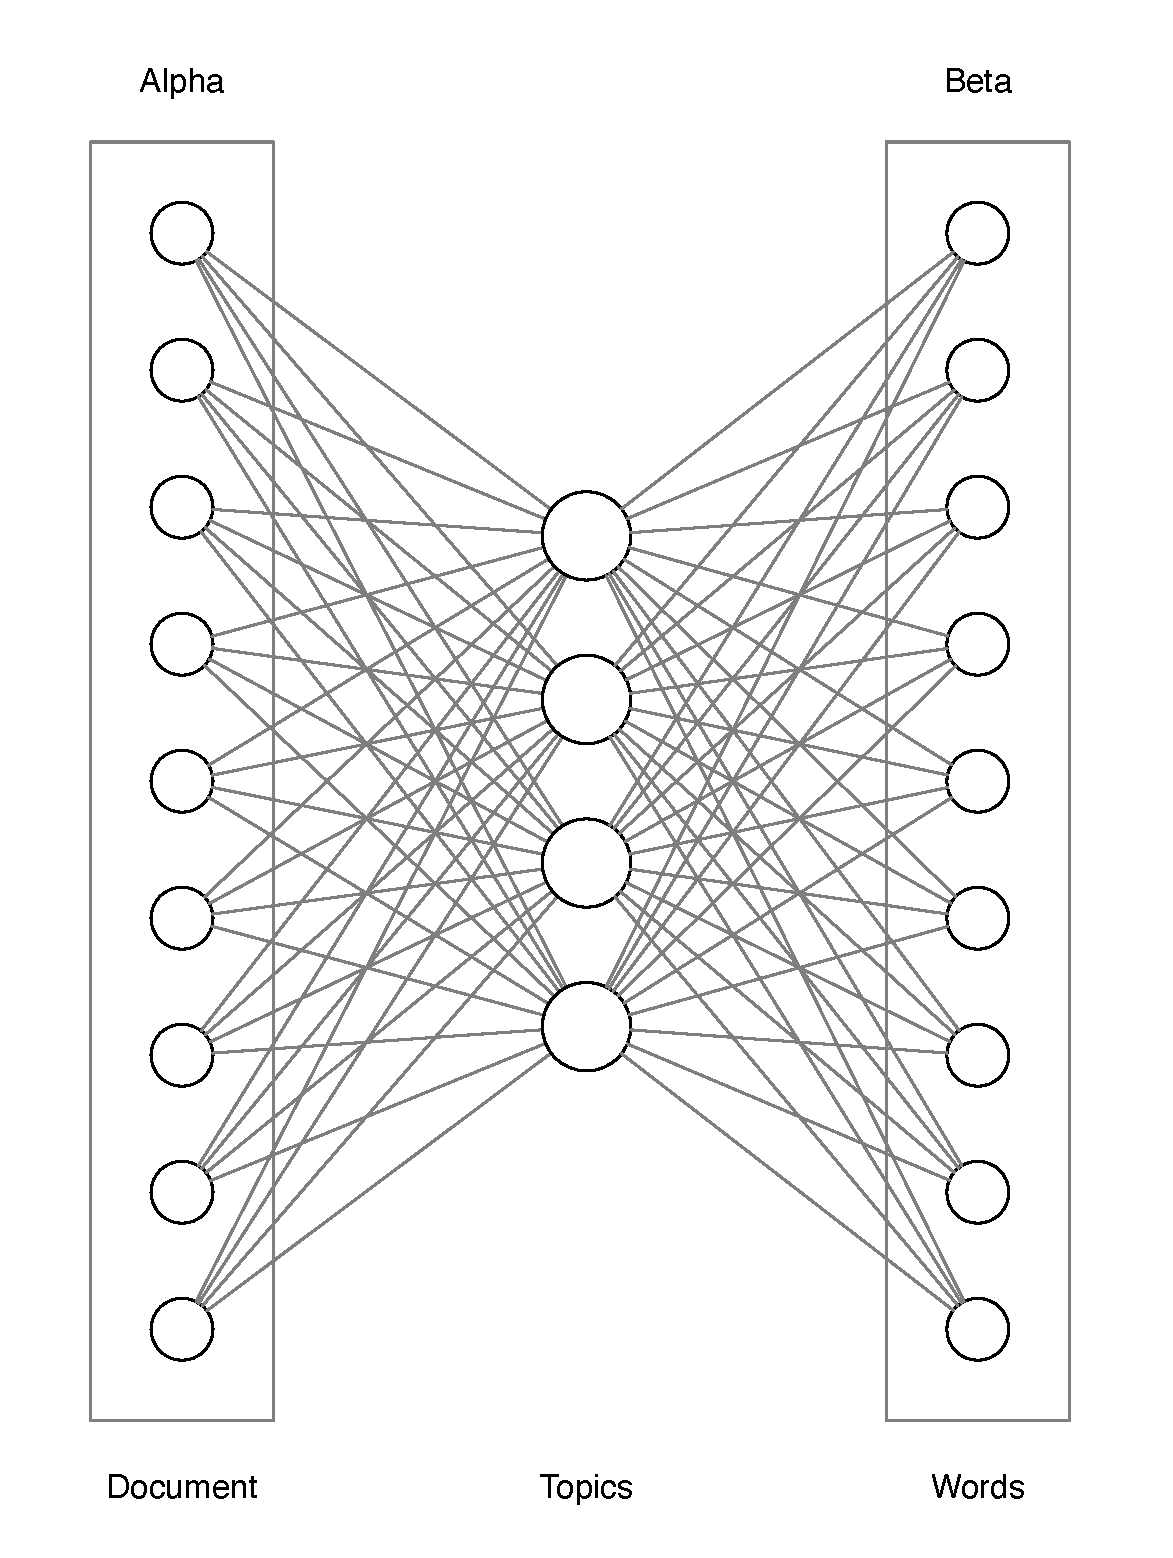
\includegraphics[width=12cm]{./figures/alpha1.eps}
\caption{Alpha and beta representation}
\label{fig:alphaandbeta}
\end{figure}

In the rest of this section, the lessons learned for both of these hyperparameters will be discussed.

\subsection{Dirichlet hyperparameter alpha}

Choosing a value of alpha or beta (eta) can be a tricky task, since these two hyperparameters have an direct impact on the topic modeling results. A high alpha means the documents contain more topics.

The researcher experimented with various alpha values. These values were 0.01, 0.1, and 0.5. It was discovered that using the above-mentioned values, the actual prototype was displaying run time divided by zero errors. The cause of the errors was linked to the alpha and beta values. The model was producing explicit zero results. 

As \citeA{wallach2009rethinking} mention, an alpha asymmetric is good, but an asymmetric beta is not. It was because of the run time errors that it was decided to set the parameters to auto. This means that the model learns an asymmetric statistical inference, or prior for short.
The hyperparameter beta will be discussed in the next sub-section.

\subsection{Dirichlet hyperparameter beta}

It was also found that experimenting with various beta (eta) values rendered the same run time errors observed with the alpha testing. The researcher also decided to set the hyperparameter to auto, which learns asymmetric prior from the data.

This approach of setting the hyperparameters to auto, as stated, was found to benefit the topics generated by the LDA model. Giving the ability to the data to learn their own prior meant that it should deliver similar results each time the model ran. Capping or limiting the hyperparameters would result in run time errors and skewed results.

As mentioned by \citeA{griffiths2004finding}, when working with scientific documents, it is best to use a larger beta (eta) value. The reason is that it could lead to the model containing a smaller number of topics and could cover more scientific concepts. This is in contrast to using a smaller beta (eta) value, which would produce more topics that would address specific concepts.

In the next section, similarities will be discussed between the probability distributions.

\section{Similarity between probability distributions}

In this section, lessons learned will be shared on the process of finding the similarities between the documents.

In Section \ref{JSD}, Jensen-Shannon Divergence (JSD) was mentioned to be the improved method used to measure similarity between two probability distributions. The researcher used the Jensen-Shannon Divergence method to calculate the distance between the two probability distributions. In recent years, research has indicated that JSD still has relevance today \cite{tong2016text,giles2019subject,he2015topic,chu2010topic}.

As there are no parameters with Jensen-Shannon Divergence, this made it easy to implement it into the prototype and ultimately, to look at the end results. Since the goal of this research was not to compare other similarity measurement methods, the researcher only considered JSD.

In the next section, evaluating the output of the similarity of the probability distributions will be discussed.

\section{Evaluation} \label{ssec:eval}

In this section the observations will be discussed between the test document and training documents. Observations will be shared to understand whether and what made the similarity list good or bad. In the next subsection a single test document with its corresponding list of similar documents will be discussed. 

The layout of the subsection will include observations on what made a topic like digital forensics and similar documents good, what LDA parameters could contribute to the change of similar documents, and how many documents matched. This structure will continue with what was considered a good match and what a bad match.

In addition to the layout of the subsections, two topics were selected to demonstrate the prototype and model. More topics were used in the experiment, however, these two topics were selected to illustrate the lessons which were learned during the study. Data related to the the other topics can be viewed in Appendix \ref{appendix: Appendix A}.

\subsection{Digital Forensics}

The title of the test document was ‘Towards a Framework for Enhancing Potential Digital Evidence Presentation’. The contents of the document covered working towards a framework to develop methodologies and specifications. The ultimate goal is to enhance the presentation and interpretation of any legal proceedings effectively.

The recommendation list of documents of the above topic consists of five documents. The list of recommendations are listed in Table \ref{tab:digitalforensics}. Observing the list, one could argue that the topic, digital forensics, was a good topic to test with.

\begin{table}[]
\centering
\resizebox{\textwidth}{!}{%
\begin{tabular}{|l|l|}
\hline
\textbf{JSD SCORE} & \textbf{TITLE} \\ \hline
0.5372 & Towards a digital forensic science \\ \hline
0.6170 & A model for secure value-added service subscriptions in cellular networks \\ \hline
0.6172 & \begin{tabular}[c]{@{}l@{}}POPI act - Opt-in and opt-out compliance from a data \\ Value chain perspective: A South African insurance industry experiment\end{tabular} \\ \hline
0.6179 & Team formation in digital forensics \\ \hline
0.6306 & The current state of digital forensic practitioners in South Africa \\ \hline
\end{tabular}%
}
\caption{Digital forensic similarity}
\label{tab:digitalforensics}
\end{table}

The researcher observed that one of the reasons that digital forensics was a good topic to test with was that there were multiple documents covering the same topic. This meant that the LDA model had more training data. Having multiple documents covering the same topic provided more words for the bag of words representation of the text.

Another observation was that since Jensen-Shannon Divergence had no real parameters to adjust, little difference could be made in the greater scheme of things. The majority of the tweaking and working must be done before getting to the Jensen-Shannon Divergence. The tweaking was done in the text pre-processing, text representation, and LDA model phases of the experiment.

\begin{lesson}[JSD no parameters]
Jensen-Shannon Divergence (JSD) does not have parameters to refine, thus putting more emphasis on the refinement of the pre-processing and topic modeling components.
\end{lesson}\label{L:JSD}

In terms of changing the LDA parameters, it was observed that increasing the chunksize of the LDA model to cover all the documents in the training set yielded good results for this specific topic. In addition, increasing the number of passes during training also yielded good results.

In the next subsection, the topic privacy, similarity list and observations will be discussed.

\subsection{Privacy}

The test document that was used had the title ‘Computer monitoring in the 21st century workplace’ which laid the foundation for a workplace privacy policy that protects employees.

The recommendation list has also provided the top five documents which it considers very similar to the document above. As viewed in Table \ref{tab:digitalforensicsBA}, the titles of the documents do not indicate any privacy topics.

\begin{table}[]
\centering
\resizebox{\textwidth}{!}{%
\begin{tabular}{|l|l|}
\hline
\textbf{JSD SCORE} & \textbf{TITLE} \\ \hline
0.5612 & A profile of the distance computing student softlifter \\ \hline
0.5820 & CDMA in signal encyption and information security \\ \hline
0.6670 & Context aware mobile application for mobile devices \\ \hline
0.6671 & Towards a framwork for a network warfare capability \\ \hline
0.6676 & Adaptable exploit detection through scalable netflow analysis \\ \hline
\end{tabular}%
}
\caption{Privacy similarity}
\label{tab:digitalforensicsBA}
\end{table}

The main observation for this subsection is that words that would be more easily identifiable in the LDA model became lost in the pre-processing and LDA pipeline.

The other observation was that once the number of topics increased, it created room for the other topics also to be included. Those topics were previously the second- or third-tier topics in the LDA model.

\begin{lesson}[More is not better]
Increasing the number of topics increases the risk that topics will be included that do not provide any significant value.
\end{lesson}\label{L:more}

As simple as it may sound, compared to digital forensics, there were not many documents which dealt with privacy and workforce topics.

\section{Summary}

In this chapter, we discussed several themes while developing the prototype. What changes were needed to be made for the prototype to perform at its maximum? The other theme was the lessons that were learned while administering the changes.

The lessons learned from each component, as indicated in Figure \ref{fig:prototype}, are summarised and shared in Table \ref{tab:lessons}. The conclusion that is drawn is that pre-processing is certainly one of the most important legs in the pipeline and needs to have most of the time dedicated to it. Each component of the pre-processing process needs to be closely considered. Removing too many words can cause documents not to any similarity to others and leaving too many words can make the LDA model too sensitive.

The experimentation, analysis, and discussion enabled the creation of the model used in Chapter \ref{chap: Chapter 6}. The model outlines the steps that were needed to achieve a recommendation list. It also opened discussions so that researchers can further the research by using additional techniques and algorithms, which will be discussed in the next chapter.

\begin{table}[htb]
\begin{tabularx}{\textwidth}{|l|X|}
\hline
\textbf{Lesson name} & \textbf{Lesson} \\ \hline
1. Goldilock's dilemma & The identification and removal of stopwords is a very important part of the pre-processing pipeline. Removing too many domain-specific words negatively influences the quality of the topics and ultimately, influences the similarity scores. \\ \hline
2. Problematic ligature characters & Researchers using different tools for typesetting can make the pre-processing pipeline exclude words containing ligature characters. \\ \hline
3. Manual intervention & When evaluating the quality of the topics generated by the model, even though evaluation techniques like coherence scores or perplexity indicate good topics, manual intervention is still needed to validate them. \\ \hline
4. Quality over quantity & Increasing the number of passes does not automatically increase the quality of the topics. \\ \hline
5. Chunksize has little influence & Increasing the chunksize does not have a significant influence on the quality of the topics. \\ \hline
6. Probability Dilemma & If the minimum probability is set too high, the topic model runs the risk of not including certain topics. Smaller documents often only have a few sentences, which influences the probability of a word occurring. Therefore, the minimum probability cannot be too high. \\ \hline
7. Flatten the curve & The perplexity score will flatten out as the number of topics gradually increase. \\ \hline
8. JSD no parameters & Jensen-Shannon Divergence (JSD) does not have parameters to refine, putting more emphasis on the refinement of the pre-processing and topic modeling components. \\ \hline
9. More is not better & Increasing the number of topics increases the risk that topics will be included that do not provide any significant value. \\ \hline
\end{tabularx}
\caption{Summary of the lessons learned}
\label{tab:lessons}
\end{table}
 
